
\begin{figure}[H]
  \centering
  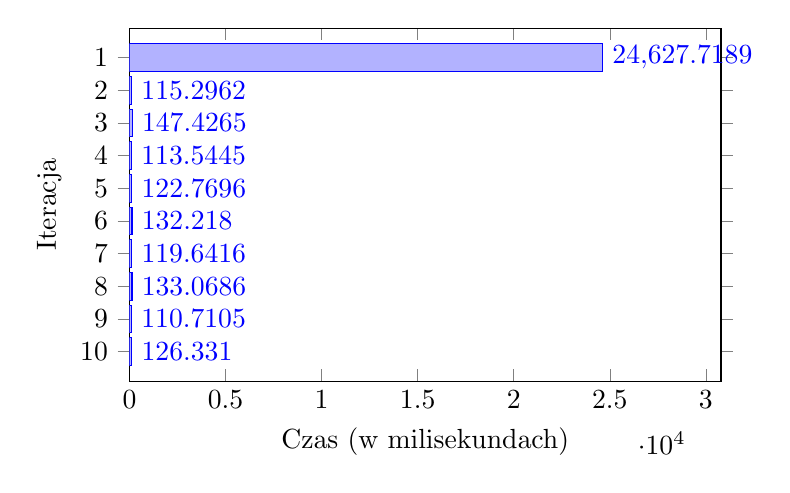
\begin{tikzpicture}
  
    \begin{axis} [
      xbar = .05cm,
      nodes near coords,
      nodes near coords style={
        /pgf/number format/precision=4,
      },
      xmin = 0,
      ytick = data,
      enlarge x limits = {value = .25, upper},
      symbolic y coords = {10,9,8,7,6,5,4,3,2,1},
      xlabel=Czas (w milisekundach),
      ylabel=Iteracja,
      width=0.75\textwidth,
      height=0.5\textwidth
    ]
    
      \addplot coordinates {(24627.718899965286,1) (115.29619997739792,2) (147.4264999628067,3) (113.54450005292892,4) (122.76960003376007,5) (132.2179999947548,6) (119.64160001277924,7) (133.06859999895096,8) (110.71050000190735,9) (126.3309999704361,10)};
      
    \end{axis}
  
  \end{tikzpicture}
  \caption{Wynik testów przykładu 10 [\ref{lst:wydajnosc-przyklad-p-10}]}
  \label{fig:wynik-przyklad-9}
\end{figure}
